% Outline slides. Compile: pdflatex quantum_sim_adiabatic_skeleton.tex
\documentclass[
	11pt,
	aspectratio=169,
	compress,
]{beamer}

\graphicspath{{Images/}{./}{_pptx_extract/ppt/media/}}
\usepackage[T1]{fontenc}
\usepackage[utf8]{inputenc}
\usepackage{lmodern}
\usepackage{microtype}
\usepackage{booktabs}
\usepackage{amsmath,amssymb}
\usepackage{tikz}
\usetikzlibrary{arrows.meta,positioning,calc}

%%% Theme from Presentation/template.tex %%%
\usetheme{Madrid}
\definecolor{myRed}{RGB}{120,4,4}
\definecolor{myOrange}{RGB}{227,125,0}
\setbeamercolor*{structure}{bg=myRed!20,fg=myRed!90}
\setbeamercolor*{palette primary}{use=structure,fg=white,bg=structure.fg}
\setbeamercolor*{palette secondary}{use=structure,fg=myRed,bg=white}
\setbeamercolor*{palette tertiary}{use=structure,fg=white,bg=myRed}
\setbeamercolor{frametitle}{bg=myRed!85,fg=white}
\setbeamercolor*{titlelike}{parent=palette primary}
\setbeamercolor{section in head/foot}{fg=myOrange, bg=white}
\setbeamercolor{item projected}{bg=myOrange}
\setbeamercolor{itemize item}{fg=myOrange}
\setbeamercolor{itemize subitem}{fg=myOrange}
\setbeamercolor{button}{bg=myOrange}
\setbeamercolor{section in toc}{fg=black}
\setbeamercolor{subsection in toc}{fg=black}
\setbeamercolor{block title}{bg=myOrange, fg=white}
\setbeamercolor{block body}{bg=myOrange!20}

\usefonttheme{default}
\useinnertheme{circles}
\useoutertheme{infolines}
\setbeamertemplate{navigation symbols}{}
\setbeamertemplate{headline}{}

\title[Quantum Simulation]{Quantum Simulation:\\ From Hamiltonians to Adiabatic Computation}
\subtitle{Outline of Topics}
\author[]{}
\institute[]{}
\date[]{}

\newcommand{\outlinebox}[1]{%
	\vspace{0.25em}%
	\begin{block}{Content outline}
		#1
	\end{block}
}

\tikzset{
	sbox/.style={
		draw=myRed!65,
		rounded corners=2pt,
		align=center,
		inner sep=3pt,
		thick,
		minimum height=0.95cm,
		font=\scriptsize
	},
	sarr/.style={-{Latex[length=2mm]}, thick, myOrange}
}

\begin{document}

%========================================================
\begin{frame}[plain]
	\vfill
	\begin{center}
		{\usebeamercolor[fg]{titlelike}
		\color{myRed}\LARGE\bfseries Quantum Simulation}\\[0.45em]
		{\Large From Hamiltonians to Adiabatic Computation}\\[0.9em]
		{\large Ground states, Ising paths, and digital adiabatic methods}
	\end{center}
	\vfill
\end{frame}

%========================================================
\section{Introduction}
\begin{frame}{Table of Contents}
	\tableofcontents
\end{frame}

%--------------------------------------------------------
\begin{frame}{Motivation}
	\begin{itemize}
		\item Quantum simulation: turn a physical model into a computational task
		\item Shared language: algorithms, Hamiltonians, and implementation methods
		\item Focus of this talk: adiabatic paths for ground-state problems, with a worked Ising example
	\end{itemize}
	\outlinebox{Physical model $\to H$ $\to$ question $\to$ method $\to$ gap, runtime, and complexity.}
\end{frame}

%--------------------------------------------------------
\begin{frame}{Roadmap}
	\centering
	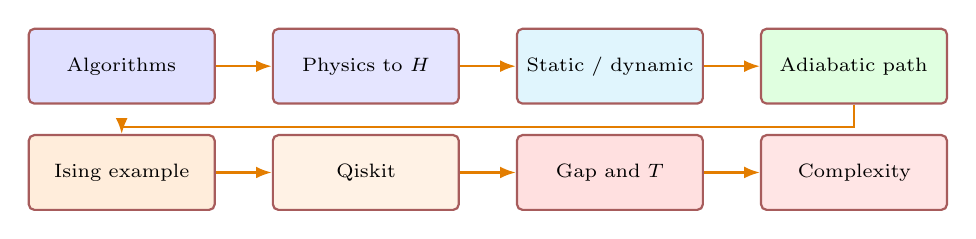
\begin{tikzpicture}[x=1cm, y=1cm]
		\node[sbox, text width=2.15cm, fill=blue!12] (a) at (0,1.35) {Algorithms};
		\node[sbox, text width=2.15cm, fill=blue!10] (b) at (3.1,1.35) {Physics to $H$};
		\node[sbox, text width=2.15cm, fill=cyan!12] (c) at (6.2,1.35) {Static / dynamic};
		\node[sbox, text width=2.15cm, fill=green!12] (d) at (9.3,1.35) {Adiabatic path};
		\node[sbox, text width=2.15cm, fill=orange!14] (e) at (0,0) {Ising example};
		\node[sbox, text width=2.15cm, fill=orange!10] (f) at (3.1,0) {Qiskit};
		\node[sbox, text width=2.15cm, fill=red!12] (g) at (6.2,0) {Gap and $T$};
		\node[sbox, text width=2.15cm, fill=red!10] (h) at (9.3,0) {Complexity};
		\draw[sarr] (a) -- (b);
		\draw[sarr] (b) -- (c);
		\draw[sarr] (c) -- (d);
		\draw[sarr] (d.south) -- ++(0,-0.28) -| (e.north);
		\draw[sarr] (e) -- (f);
		\draw[sarr] (f) -- (g);
		\draw[sarr] (g) -- (h);
	\end{tikzpicture}
	\outlinebox{Deep dive on adiabatic ground-state computation; digital primitives appear as tools for the same path.}
\end{frame}

%========================================================
\section{Algorithms and layers}
\begin{frame}{What Is an Algorithm?}
	\begin{itemize}
		\item Finite procedure: input $\to$ instructions $\to$ output
		\item Independent of a particular machine realization
		\item ``Quantum'' changes the execution model, not this definition
	\end{itemize}
	\outlinebox{Operational definition; contrast with a device-specific program.}
\end{frame}

%--------------------------------------------------------
\begin{frame}{Quantum Algorithms at a Glance}
	\begin{enumerate}
		\item State preparation on qubits
		\item Unitary evolution: gate circuits or Hamiltonian control
		\item Measurement and extraction of observables
	\end{enumerate}
	\outlinebox{Three-part skeleton only; no gate-set or circuit-depth discussion yet.}
\end{frame}

%--------------------------------------------------------
\begin{frame}{Three Layers}
	\centering
	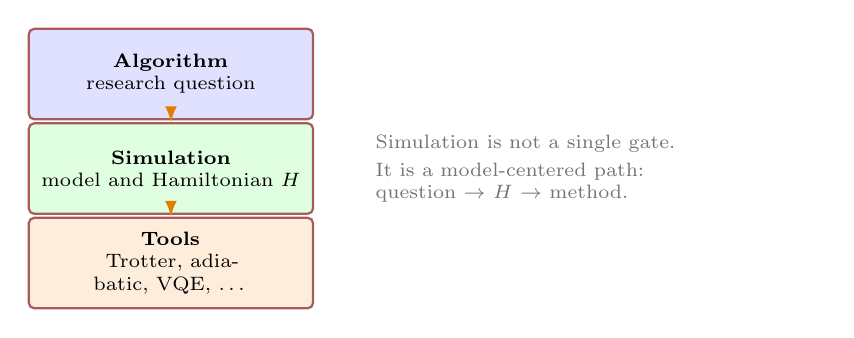
\begin{tikzpicture}[x=1cm, y=1cm]
		\node[sbox, text width=3.4cm, fill=blue!12, minimum height=1.15cm] (L1) at (0,2.2)
			{\textbf{Algorithm}\\research question};
		\node[sbox, text width=3.4cm, fill=green!12, minimum height=1.15cm] (L2) at (0,1.0)
			{\textbf{Simulation}\\model and Hamiltonian $H$};
		\node[sbox, text width=3.4cm, fill=orange!14, minimum height=1.15cm] (L3) at (0,-0.2)
			{\textbf{Tools}\\Trotter, adiabatic, VQE, \ldots};
		\draw[sarr] (L1) -- (L2);
		\draw[sarr] (L2) -- (L3);
		\node[font=\scriptsize, text=black!55, align=left, text width=5.6cm] at (5.4,1.0) {%
			Simulation is not a single gate.\\[2pt]
			It is a model-centered path:\\
			question $\to$ $H$ $\to$ method.};
	\end{tikzpicture}
	\outlinebox{Layer 1 asks; layer 2 represents the physics; layer 3 implements $U(t)$, $H(s)$, or $f(H)$.}
\end{frame}

%--------------------------------------------------------
\begin{frame}{What Quantum Simulation Means}
	\begin{itemize}
		\item Use a controllable quantum system to study another quantum model
		\item Digital, analog, or hybrid realizations
		\item Common starting point: fix $H$ and the retained degrees of freedom
	\end{itemize}
	\outlinebox{Typical models: Hubbard, molecules, spin lattices, circuit modes.}
\end{frame}

%========================================================
\section{From physics to Hamiltonians}
\begin{frame}{From Physical Problem to Mathematical Model}
	\centering
	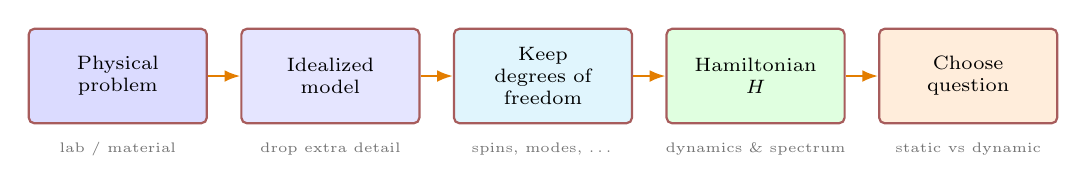
\begin{tikzpicture}[x=1cm, y=1cm]
		\node[sbox, text width=2.05cm, fill=blue!14, minimum height=1.2cm] (phys) at (0,0.7) {Physical\\problem};
		\node[sbox, text width=2.05cm, fill=blue!10, minimum height=1.2cm] (mod) at (2.7,0.7) {Idealized\\model};
		\node[sbox, text width=2.05cm, fill=cyan!12, minimum height=1.2cm] (dof) at (5.4,0.7) {Keep\\degrees of freedom};
		\node[sbox, text width=2.05cm, fill=green!12, minimum height=1.2cm] (H) at (8.1,0.7) {Hamiltonian\\$H$};
		\node[sbox, text width=2.05cm, fill=orange!14, minimum height=1.2cm] (q) at (10.8,0.7) {Choose\\question};
		\draw[sarr] (phys) -- (mod);
		\draw[sarr] (mod) -- (dof);
		\draw[sarr] (dof) -- (H);
		\draw[sarr] (H) -- (q);
		\node[font=\tiny, text=black!55, below=3pt of phys] {lab / material};
		\node[font=\tiny, text=black!55, below=3pt of mod] {drop extra detail};
		\node[font=\tiny, text=black!55, below=3pt of dof] {spins, modes, \ldots};
		\node[font=\tiny, text=black!55, below=3pt of H] {dynamics \& spectrum};
		\node[font=\tiny, text=black!55, below=3pt of q] {static vs dynamic};
	\end{tikzpicture}
	\vspace{0.35em}
	\outlinebox{A model is a deliberate compression: what is kept versus discarded.}
\end{frame}

%--------------------------------------------------------
\begin{frame}{Representative Physical Problems}
	\renewcommand{\arraystretch}{1.25}
	\begin{center}
	\small
	\begin{tabular}{@{}lll@{}}
		\toprule
		\textbf{Physical setting} & \textbf{Typical model} & \textbf{Degrees of freedom} \\
		\midrule
		Magnets / spin glasses & Ising / Heisenberg & spins on a lattice \\
		Correlated electrons & Hubbard & electrons + spin \\
		Molecules & electronic structure & active orbitals \\
		Cavities / circuits & oscillator / LC & flux and charge \\
		\bottomrule
	\end{tabular}
	\end{center}
	\outlinebox{The same material can map to different models, depending on the question.}
\end{frame}

%--------------------------------------------------------
\begin{frame}{Classical and Quantum Roles of $H$}
	\begin{columns}[T]
		\begin{column}{0.48\textwidth}
			\begin{block}{Classical}
				\begin{itemize}
					\item Energy on phase space
					\item Generator of motion
					\item Minimization $\neq$ dynamics
				\end{itemize}
			\end{block}
		\end{column}
		\begin{column}{0.48\textwidth}
			\begin{block}{Quantum}
				\begin{itemize}
					\item Spectrum: $\hat H\lvert E_n\rangle=E_n\lvert E_n\rangle$
					\item Dynamics: $i\hbar\,\partial_t\lvert\psi\rangle=\hat H\lvert\psi\rangle$
					\item Same dual role continues
				\end{itemize}
			\end{block}
		\end{column}
	\end{columns}
	\vspace{0.35em}
	\outlinebox{Almost every simulation task is a function of one Hamiltonian: $e^{-iHt}$, ground state, or $H(s)$.}
\end{frame}

%--------------------------------------------------------
\begin{frame}{Why $H$ Is Central in Simulation}
	\begin{itemize}
		\item Fix the model and $H$ first; then choose the question and the method
		\item Tools (Trotter, adiabatic, VQE) come after the representation is clear
		\item Choosing a method before fixing $H$ is premature
	\end{itemize}
	\outlinebox{This talk keeps the Hamiltonian language primary.}
\end{frame}

%========================================================
\section{Static and dynamic problems}
\begin{frame}{Two Questions from One Hamiltonian}
	\centering
	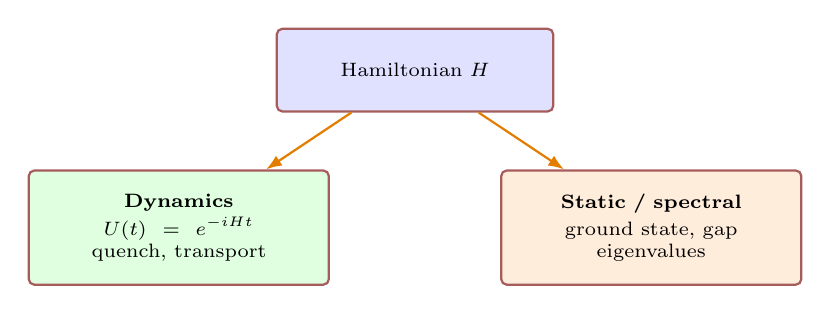
\begin{tikzpicture}[x=1cm, y=1cm]
		\node[sbox, text width=3.3cm, fill=blue!12, minimum height=1.05cm] (H) at (4.6,2.15) {Hamiltonian $H$};
		\node[sbox, text width=3.6cm, fill=green!12, minimum height=1.45cm] (dyn) at (1.6,0.15) {%
			\textbf{Dynamics}\\[2pt]
			$U(t)=e^{-iHt}$\\
			quench, transport};
		\node[sbox, text width=3.6cm, fill=orange!14, minimum height=1.45cm] (stat) at (7.6,0.15) {%
			\textbf{Static / spectral}\\[2pt]
			ground state, gap\\
			eigenvalues};
		\draw[sarr] (H) -- (dyn);
		\draw[sarr] (H) -- (stat);
	\end{tikzpicture}
	\vspace{0.2em}
	\outlinebox{The same $H$ supports two research paths. This talk follows the static / ground-state branch.}
\end{frame}

%--------------------------------------------------------
\begin{frame}{Ground-State Problems: Why They Matter}
	\begin{itemize}
		\item Lowest-energy configuration of a physical model (magnetism, molecules, lattices)
		\item Many optimization tasks map to Ising / QUBO ground states
		\item Spectral gap and low-lying excitations control both physics and runtime
	\end{itemize}
	\begin{alertblock}{Target for the rest of the talk}
		Prepare / identify the ground state of a problem Hamiltonian $H_P$.
	\end{alertblock}
\end{frame}

%--------------------------------------------------------
\begin{frame}{Two Main Approaches}
	\begin{enumerate}
		\item \textbf{Time evolution:} build or approximate $e^{-iHt}$ or $f(H)$
		\item \textbf{Adiabatic:} slow path $H_{\mathrm{init}}\to H_P$, stay in the instantaneous ground state
	\end{enumerate}
	\begin{block}{Focus ahead}
		Adiabatic computation, a two-qubit Ising example, Qiskit implementation, then gap, runtime, and complexity.
	\end{block}
	\outlinebox{Trotter appears later as a digital tool for the same adiabatic path.}
\end{frame}

%========================================================
\section{Adiabatic computation}
\begin{frame}{Adiabatic Idea in One Slide}
	\begin{enumerate}
		\item Start from an easy initial Hamiltonian $H_{\mathrm{init}}$ ($H_B$) with a known ground state
		\item Interpolate slowly to the problem Hamiltonian $H_P$
		\item Sufficient gap and time $\Rightarrow$ ground state of $H_P$
	\end{enumerate}
	\outlinebox{Encode the problem in a Hamiltonian path rather than enumerating configurations.}
\end{frame}

%--------------------------------------------------------
\begin{frame}{The Path $H(s)$}
	\begin{itemize}
		\item Standard linear interpolation
		\[
			H(s)=(1-s)\,H_{\mathrm{init}} + s\,H_P,\qquad 0\le s\le 1
		\]
		\item Example schedule: $s(t)=t/T$
		\item $s$ mixes the two Hamiltonians; it is not itself physical time
	\end{itemize}
	\outlinebox{$H(s)$ is linear in $s$; the eigenvalues generally are not.}
\end{frame}

%--------------------------------------------------------
\begin{frame}{Instantaneous Gap and Runtime $T$}
	\begin{columns}[T]
		\begin{column}{0.48\textwidth}
			\begin{itemize}
				\item $\Delta(s)=E_1(s)-E_0(s)$
				\item $\Delta_{\min}=\min_s\Delta(s)$ is the bottleneck
				\item Heuristic scale: $T\propto 1/\Delta_{\min}^{2}$
			\end{itemize}
		\end{column}
		\begin{column}{0.50\textwidth}
			\centering
			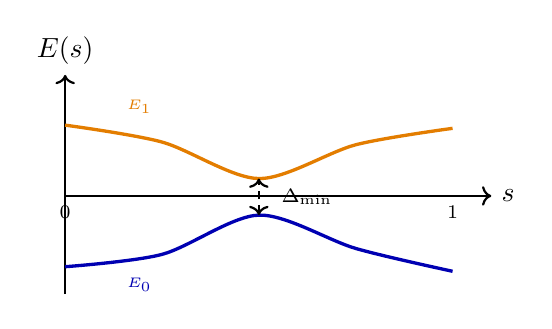
\begin{tikzpicture}[x=0.82cm, y=0.58cm]
				\draw[->, thick] (0,0) -- (6.6,0) node[right] {$s$};
				\draw[->, thick] (0,-2.15) -- (0,2.65) node[above] {$E(s)$};
				\node[below, font=\scriptsize] at (0,0) {$0$};
				\node[below, font=\scriptsize] at (6,0) {$1$};
				\draw[very thick, blue!70!black] plot[smooth] coordinates
					{(0,-1.55) (1.5,-1.28) (3,-0.42) (4.5,-1.15) (6,-1.65)};
				\draw[very thick, myOrange] plot[smooth] coordinates
					{(0,1.55) (1.5,1.18) (3,0.38) (4.5,1.12) (6,1.48)};
				\draw[<->, densely dashed, thick] (3,-0.42) -- (3,0.38);
				\node[font=\scriptsize, right] at (3.2,-0.02) {$\Delta_{\min}$};
				\node[font=\tiny, blue!70!black] at (1.15,-1.95) {$E_0$};
				\node[font=\tiny, myOrange] at (1.15,1.95) {$E_1$};
			\end{tikzpicture}
		\end{column}
	\end{columns}
	\outlinebox{Scaling estimate, not a universal theorem bound. Avoided crossing: levels approach, then separate.}
\end{frame}

%--------------------------------------------------------
\begin{frame}{Why Adiabatic for Ground States?}
	\begin{itemize}
		\item Transparent physical picture: follow the ground state along a path
		\item Natural match to analog field schedules
		\item Digitally expressible via Trotterized paths (digital adiabatic)
	\end{itemize}
	\outlinebox{Less natural when the target is a precise $e^{-iHt}$ or a general $f(H)$.}
\end{frame}

%========================================================
\section{Worked example: Ising}
\begin{frame}{Two-Qubit Setup}
	\begin{itemize}
		\item Make $H_{\mathrm{init}}$, $H_P$, the gap, and $T$ concrete
		\item System: two spin-$1/2$ particles (two qubits)
		\item Parameters: $h_x=1$, $J=1$, $h_z=1/4$
	\end{itemize}
	\outlinebox{Small enough that the full spectrum can be seen numerically.}
\end{frame}

%--------------------------------------------------------
\begin{frame}{Initial Hamiltonian $H_B$}
	\begin{itemize}
		\item $H_B=-h_x(X_1+X_2)$ \quad ($h_x>0$)
		\item Easy ground state $\lvert++\rangle$, prepared by Hadamards on $\lvert00\rangle$
		\item Also called the driver / beginning Hamiltonian
	\end{itemize}
	\outlinebox{Transverse field; product eigenstates of $X$.}
\end{frame}

%--------------------------------------------------------
\begin{frame}{Problem Hamiltonian $H_P$}
	\begin{itemize}
		\item $H_P=-J Z_1Z_2 - h_z(Z_1+Z_2)$ \quad ($J,h_z>0$)
		\item Target ground state $\lvert00\rangle$
		\item Ferromagnetic coupling plus a longitudinal field that lifts the degeneracy
	\end{itemize}
	\outlinebox{Optimization reading: the ground configuration is the solution.}
\end{frame}

%--------------------------------------------------------
\begin{frame}{Adiabatic Pipeline for the Ising Example}
	\centering
	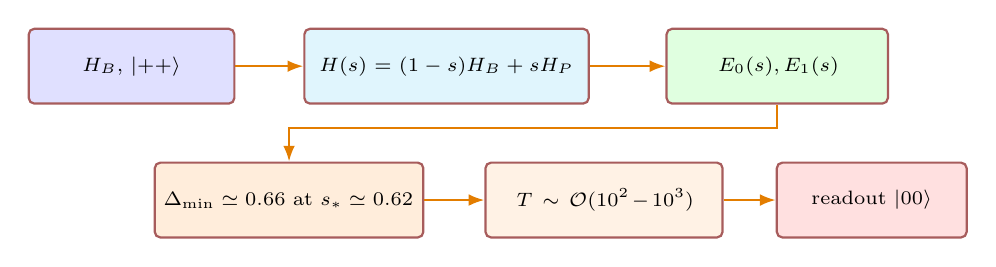
\begin{tikzpicture}[x=1cm, y=0.85cm, font=\small]
		\node[sbox, text width=2.4cm, fill=blue!12] (a) at (0,2.2) {$H_B$, $\lvert++\rangle$};
		\node[sbox, text width=3.4cm, fill=cyan!12] (b) at (4.0,2.2) {$H(s)=(1-s)H_B+sH_P$};
		\node[sbox, text width=2.6cm, fill=green!12] (c) at (8.2,2.2) {$E_0(s),E_1(s)$};
		\node[sbox, text width=3.2cm, fill=orange!14] (d) at (2.0,0.2) {$\Delta_{\min}\simeq0.66$ at $s_*\simeq0.62$};
		\node[sbox, text width=2.8cm, fill=orange!10] (e) at (6.0,0.2) {$T\sim\mathcal{O}(10^{2}\!-\!10^{3})$};
		\node[sbox, text width=2.2cm, fill=red!12] (f) at (9.4,0.2) {readout $\lvert00\rangle$};
		\draw[sarr] (a) -- (b);
		\draw[sarr] (b) -- (c);
		\draw[sarr] (c.south) -- ++(0,-0.35) -| (d.north);
		\draw[sarr] (d) -- (e);
		\draw[sarr] (e) -- (f);
	\end{tikzpicture}
	\vspace{0.3em}
	\outlinebox{Numbers from the two-qubit path; endpoint gaps alone do not locate the bottleneck.}
\end{frame}

%--------------------------------------------------------
\begin{frame}{Numerical Path Result}
	\begin{columns}[T]
		\begin{column}{0.52\textwidth}
			\begin{itemize}
				\item Gap minimum near $s_*\simeq 0.62$
				\item $\Delta_{\min}\simeq 0.66$
				\item Heuristic with $\varepsilon\sim 10^{-2}$: $T_{\mathrm{heur}}\sim 5\times 10^{2}$
				\item For $n=2$, $T\sim 40$ already yields near-unit success
			\end{itemize}
		\end{column}
		\begin{column}{0.46\textwidth}
			\centering
			\IfFileExists{_pptx_extract/ppt/media/image10.png}{%
				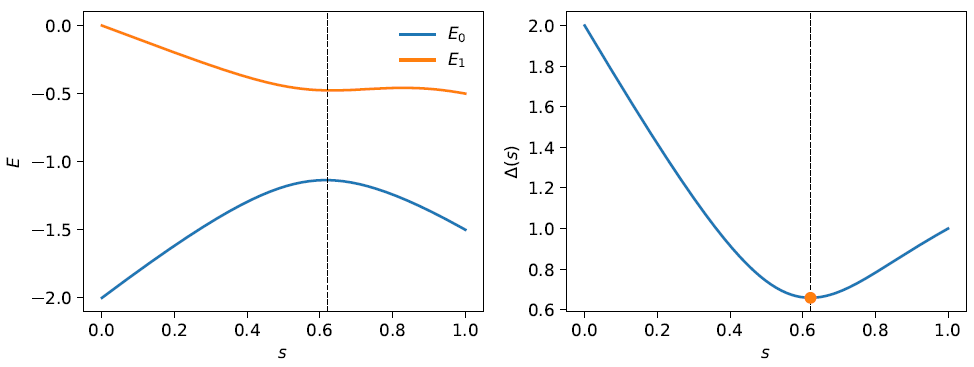
\includegraphics[width=\linewidth]{_pptx_extract/ppt/media/image10.png}%
			}{%
				\textit{(gap plot)}%
			}
		\end{column}
	\end{columns}
	\outlinebox{Distinguish a heuristic bound from a practical runtime checked by dynamics.}
\end{frame}

%========================================================
\section{Qiskit implementation}
\begin{frame}{Role of Qiskit}
	\begin{itemize}
		\item Shared implementation stack for digital circuits
		\item Turns the adiabatic path into a reproducible workflow
		\item Environment: \texttt{conda activate qcomputing}
	\end{itemize}
	\outlinebox{Close the loop from the Hamiltonian path to executable steps.}
\end{frame}

%--------------------------------------------------------
\begin{frame}{Code Steps (1): Build $H(s)$}
	\begin{enumerate}
		\item Build $H_B$ and $H_P$ with \texttt{SparsePauliOp}
		\item Form $H(s)=(1-s)H_B+sH_P$
		\item Scan $s$ and extract $\Delta_{\min}$ and $s_*$
	\end{enumerate}
	\vspace{0.2em}
	\IfFileExists{_pptx_extract/ppt/media/image11.png}{%
		\begin{center}
			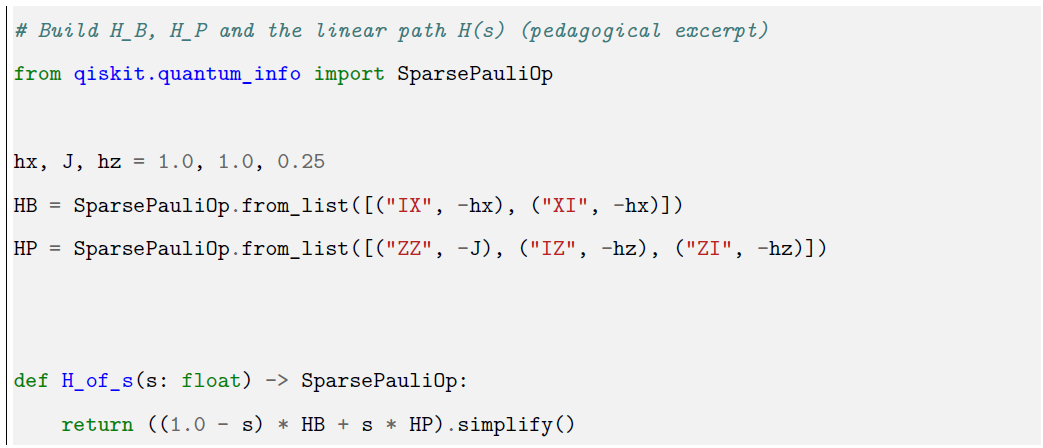
\includegraphics[height=0.42\textheight]{_pptx_extract/ppt/media/image11.png}
		\end{center}
	}{}
	\outlinebox{Scripts in \texttt{snippets/adi\_ising\_*.py} / notebook.}
\end{frame}

%--------------------------------------------------------
\begin{frame}{Code Steps (2): Trotter Layer and Readout}
	\centering
	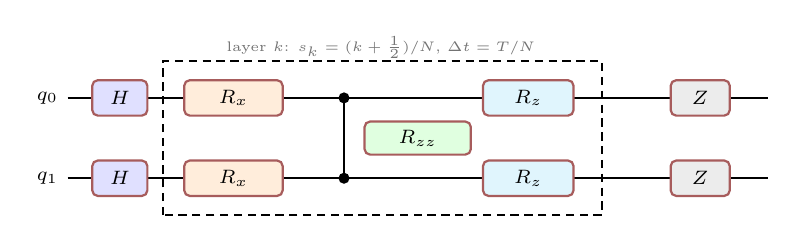
\begin{tikzpicture}[x=0.78cm, y=0.85cm]
		\draw[thick] (0,1.6) -- (11.4,1.6);
		\draw[thick] (0,0.4) -- (11.4,0.4);
		\node[left, font=\scriptsize] at (0,1.6) {$q_0$};
		\node[left, font=\scriptsize] at (0,0.4) {$q_1$};
		\node[sbox, fill=blue!12, minimum width=0.7cm, minimum height=0.45cm] at (0.85,1.6) {$H$};
		\node[sbox, fill=blue!12, minimum width=0.7cm, minimum height=0.45cm] at (0.85,0.4) {$H$};
		\draw[thick, densely dashed] (1.55,-0.15) rectangle (8.7,2.15);
		\node[font=\tiny, text=black!55] at (5.1,2.35) {layer $k$: $s_k=(k+\tfrac12)/N$, $\Delta t=T/N$};
		\node[sbox, fill=orange!14, minimum width=1.25cm, minimum height=0.45cm] at (2.7,1.6) {$R_x$};
		\node[sbox, fill=orange!14, minimum width=1.25cm, minimum height=0.45cm] at (2.7,0.4) {$R_x$};
		\fill (4.5,1.6) circle (2pt);
		\fill (4.5,0.4) circle (2pt);
		\draw[thick] (4.5,1.6) -- (4.5,0.4);
		\node[sbox, fill=green!12, minimum width=1.35cm, minimum height=0.42cm] at (5.7,1.0) {$R_{zz}$};
		\node[sbox, fill=cyan!12, minimum width=1.15cm, minimum height=0.45cm] at (7.5,1.6) {$R_z$};
		\node[sbox, fill=cyan!12, minimum width=1.15cm, minimum height=0.45cm] at (7.5,0.4) {$R_z$};
		\node[sbox, fill=gray!15, minimum width=0.75cm, minimum height=0.45cm] at (10.3,1.6) {$Z$};
		\node[sbox, fill=gray!15, minimum width=0.75cm, minimum height=0.45cm] at (10.3,0.4) {$Z$};
	\end{tikzpicture}
	\vspace{0.25em}
	\begin{itemize}
		\item $a=(1-s)h_x\Delta t$,\quad $b=s J\Delta t$,\quad $c=s h_z\Delta t$
		\item Prepare $\lvert++\rangle$, apply layers, measure in the $Z$ basis
	\end{itemize}
\end{frame}

%--------------------------------------------------------
\begin{frame}{Sample Execution Outcome}
	\begin{itemize}
		\item With $T=40$ and $N=200$: $P(\lvert00\rangle)\approx 0.9999$
		\item Aer shots concentrate on the bitstring \texttt{00}
		\item The same run produces the path-gap plot
	\end{itemize}
	\outlinebox{Success probability is a check of the digital adiabatic schedule.}
\end{frame}

%========================================================
\section{Gap and required time}
\begin{frame}{Gap Vocabulary}
	\begin{itemize}
		\item \textbf{Instantaneous gap:} $\Delta(s)=E_1(s)-E_0(s)$
		\item \textbf{Minimum gap:} $\Delta_{\min}=\min_s\Delta(s)$ --- the bottleneck
		\item \textbf{Avoided crossing:} levels approach then separate without crossing
		\item Full gap versus the gap inside a reachable symmetry sector
	\end{itemize}
	\outlinebox{The smallest spectral distance alone is not a sufficient criterion.}
\end{frame}

%--------------------------------------------------------
\begin{frame}{Three Meanings of Required Time}
	\begin{enumerate}
		\item Heuristic / order-of-magnitude estimate ($T\sim 1/\Delta_{\min}^{2}$)
		\item Sufficient bound under explicit assumptions
		\item Practical time from dynamics and a success threshold
	\end{enumerate}
	\outlinebox{These three numbers usually disagree.}
\end{frame}

%--------------------------------------------------------
\begin{frame}{Scheduling: Linear or Nonlinear}
	\begin{columns}[T]
		\begin{column}{0.48\textwidth}
			\begin{itemize}
				\item Linear: $s(t)=t/T$
				\item Nonlinear: slow down near the bottleneck
				\item Same path $H(s)$, different speed through $s$
				\item Spend more time where $\Delta(s)$ is smallest
			\end{itemize}
		\end{column}
		\begin{column}{0.50\textwidth}
			\centering
			\IfFileExists{_pptx_extract/ppt/media/image17.png}{%
				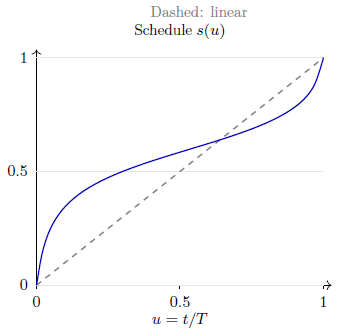
\includegraphics[height=0.55\textheight]{_pptx_extract/ppt/media/image17.png}%
			}{%
				\begin{tikzpicture}[x=2.2cm, y=2.2cm]
					\draw[->] (0,0) -- (1.15,0) node[right] {$u=t/T$};
					\draw[->] (0,0) -- (0,1.15) node[above] {$s(u)$};
					\draw[dashed, gray] (0,0) -- (1,1);
					\draw[thick, blue!70!black] plot[smooth] coordinates
						{(0,0) (0.25,0.18) (0.5,0.5) (0.75,0.82) (1,1)};
				\end{tikzpicture}%
			}
		\end{column}
	\end{columns}
\end{frame}

%========================================================
\section{Complexity and scaling}
\begin{frame}{Scaling Chain}
	\begin{equation*}
		n
		\longrightarrow
		H_n(s)
		\longrightarrow
		\Delta_{\min}(n)
		\longrightarrow
		T(n)
		\longrightarrow
		\text{complexity}
	\end{equation*}
	\begin{itemize}
		\item Qubit count alone is not a measure of difficulty
		\item The family $H_n(s)$ decides how the gap closes
	\end{itemize}
	\outlinebox{Two problems with the same $n$ can have completely different adiabatic costs.}
\end{frame}

%--------------------------------------------------------
\begin{frame}{Polynomial vs.\ Exponential Gap Closing}
	\begin{columns}[T]
		\begin{column}{0.52\textwidth}
			\begin{itemize}
				\item Polynomial: $\Delta_{\min}(n)\sim n^{-\alpha}$ $\Rightarrow$ $T\sim n^{2\alpha}$
				\item Exponential: $\Delta_{\min}(n)\sim e^{-cn}$ $\Rightarrow$ $T\sim e^{2cn}$
				\item Polynomial closing is the scalable regime for adiabatic methods
			\end{itemize}
		\end{column}
		\begin{column}{0.46\textwidth}
			\centering
			\IfFileExists{_pptx_extract/ppt/media/image14.png}{%
				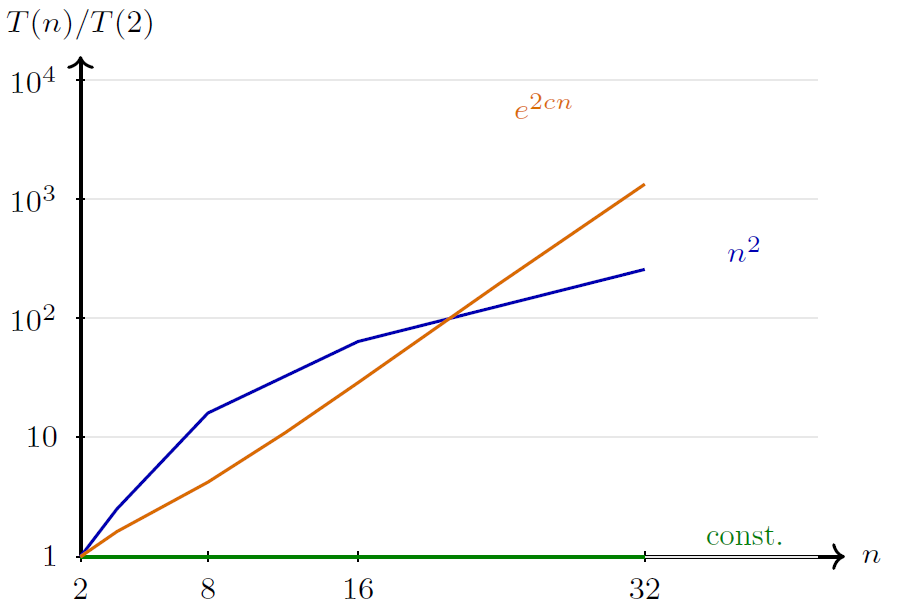
\includegraphics[width=\linewidth]{_pptx_extract/ppt/media/image14.png}%
			}{}
		\end{column}
	\end{columns}
	\outlinebox{Relative runtime $T(n)/T(2)$: constant, $n^{2}$, and $e^{2cn}$ regimes.}
\end{frame}

%--------------------------------------------------------
\begin{frame}{Three Typical Regimes}
	\renewcommand{\arraystretch}{1.2}
	\begin{center}
	\small
	\begin{tabular}{@{}lll@{}}
		\toprule
		\textbf{Family} & \textbf{Gap} & \textbf{Typical $T$} \\
		\midrule
		Only initial $H_B$ & $\Delta=2h_x$ (indep.\ of $n$) & $T$ independent of $n$ \\
		Critical TFIM (open) & $\Delta\sim 1/n$ & $T\sim n^{2}$ \\
		Tunneling / ordered phase & $\Delta\sim e^{-cn}$ & $T\sim e^{2cn}$ \\
		\bottomrule
	\end{tabular}
	\end{center}
	\vspace{0.3em}
	\outlinebox{Times are scaling estimates $T\sim\hbar/\Delta_{\min}^{2}$, not theorem bounds.}
\end{frame}

%--------------------------------------------------------
\begin{frame}{Three Complexity Layers}
	\begin{enumerate}
		\item Hardness of the \textbf{ground-state problem}
		\item Hardness of a \textbf{particular adiabatic path}
		\item Cost of a \textbf{digital implementation} of that path
	\end{enumerate}
	\begin{alertblock}{Message}
		Keep these three layers separate when assessing feasibility.
	\end{alertblock}
\end{frame}

%========================================================
\section{Challenges and summary}
\begin{frame}{What Limits Adiabatic Simulation in Practice}
	\begin{itemize}
		\item Gap closing with system size (polynomial vs.\ exponential)
		\item Control / scheduling near the bottleneck
		\item Noise and symmetry breaking along analog or digital paths
		\item Trotterization error and circuit depth in digital implementations
	\end{itemize}
	\outlinebox{Related routes for the same $H_P$: QAOA, VQE --- different method, same model.}
\end{frame}

%--------------------------------------------------------
\begin{frame}{Key Takeaways}
	\begin{enumerate}
		\item Simulation starts by fixing $H$ and the degrees of freedom
		\item Static and dynamic questions are distinct for the same $H$
		\item Adiabatic computation is a path $H(s)$; the gap sets the time
		\item Complexity follows $\Delta_{\min}(n)$ and the problem class, not $n$ alone
		\item Worked Ising + Qiskit make the gap and runtime concrete
	\end{enumerate}
\end{frame}

%--------------------------------------------------------
\begin{frame}{Outlook}
	\begin{itemize}
		\item Adaptive schedules that slow down near a small gap
		\item Scaling studies beyond $n=2$ (TFIM families)
		\item Comparison with variational routes such as QAOA and VQE
	\end{itemize}
	\outlinebox{Related notes: \texttt{QS\&QA\_Fundation/QS\&QA\_Fundation.tex}}
\end{frame}

%========================================================
\appendix
\setbeamertemplate{headline}{}
\addtobeamertemplate{frametitle}{\vspace*{-\headheight}}{}

\begin{frame}[plain,noframenumbering]
	\begin{center}
		{\LARGE Questions}
	\end{center}
\end{frame}

\end{document}
